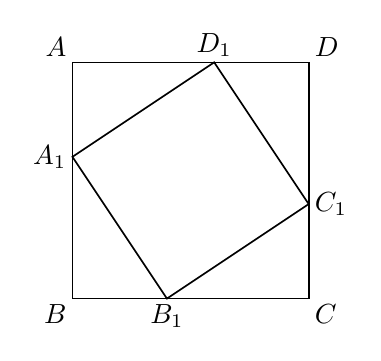
\begin{tikzpicture}[x=1cm,y=1cm,font=\normalsize,
 geometry edge/.style={solid,line width=.6pt},
 geometry mark/.style={solid,line width=.6pt},
 geometry label/.style={font=\normalsize,inner sep=2pt}]
\coordinate (A) at (0,3);
\coordinate (B) at (0,0);
\coordinate (C) at (3,0);
\coordinate (D) at (3,3);
\coordinate (A1) at (0,1.8);
\coordinate (B1) at (1.2,0);
\coordinate (C1) at (3,1.2);
\coordinate (D1) at (1.8,3);
\draw[geometry edge] (A)--(B)--(C)--(D)--cycle;
\draw[geometry edge] (A1)--(B1)--(C1)--(D1)--cycle;
\node[geometry label,above left] at (A) {$A$};
\node[geometry label,below left] at (B) {$B$};
\node[geometry label,below right] at (C) {$C$};
\node[geometry label,above right] at (D) {$D$};
\node[geometry label,left] at (A1) {$A_1$};
\node[geometry label,below] at (B1) {$B_1$};
\node[geometry label,right] at (C1) {$C_1$};
\node[geometry label,above] at (D1) {$D_1$};
\end{tikzpicture}
